%! TEX root = diss.tex
\documentclass[../diss.tex]{subfiles}
\chapter{Evaluation}

% ** Success criteria **
%
% (1) MatMul-based algo, find shortet path, can give list of nodes
%  * Manualled created resulted for some set of example graphs (see appendix)
%  * Also implemented serial dijkstra routine that is simple to prove
%    correctness of, and compared the result on $362^2$ possible pair paths on a
%    random large graph, as a unit test. Gives same results
%  * Show example list of nodes, and can make a simple plot on the California
%    road network, on compressed graph, showing a long path...
% (2) MatMul routine parallelised, runs on parallel simulation,
%     each PE can send data
%  * Unit tests for this interface, first show interface working
%  * Show `FoxOtto`, `GeneralisedFoxOtto` and corresponding unit tests
%  * Further evidence of correctness is correctness test for paths, The paths
%    found are unlikely to be correct if the matrix mult. routine is faulty
% (3) Routine minimises amount of data movement
%  * FoxOtto technique is used,
%  * Looking at code, we only send over a single interconnect, so all the data
%    is in the right location after moving it only once. This is clearly
%    minimal if we do not have shared memory. Additionally, no congested
%    interconnect as this would throw `....`
%  (? Table with counts for the number of memory movements in total? ?)
% (4) High parallel efficiency for solving APSP
%  * Refer back to equation 2.3 in section 2.1 about computation ratio, then
%    refer to the computation ratio plots and say that high parallel efficeincy,
%    above 90% when problem suffcienctly sub-divided
%
% ** Other points **
% All unit tests passed (screenshot)
% Some points to show:
% * Exploits parallelism for simulation (was close to 800% CPU usage when `htop`)
% * Very expressive interface, and also raised exceptions like ..., when misused,
%   made development of parallel algorithm a lot easier
% * Extension: Generalized FoxOtto, ran on the same tests, and still produce
%   correct results (unit tests again)
% * Extension: MIMD timing simulation, unit tests
% * Extension: Graph compression, also not just mapped queries to reduced graph and give
%     path length, but also reconstruct list of nodes in original graph.
%     Reference figure as an example
% * Paragraph discussing main plot... TODO: what to say about this?
% * The whole thing about mapping onto real-hardware to do sensitivity analysis
% * Asymptotic complexity of algorithm

% Parallel MatSquare { {{
\section{Parallel MatSquare}%
\label{sec:Parallel MatSquare}

Introduction. I successfully implemented the \ac{MatSquare} algorithm. To test
the correctness, I set up several unit tests using small graphs where I manually
set up the model answer. See ...
According to the first success criteria, ...., also able to give list of nodes.




\begin{wrapfigure}{r}{0.5\textwidth}
    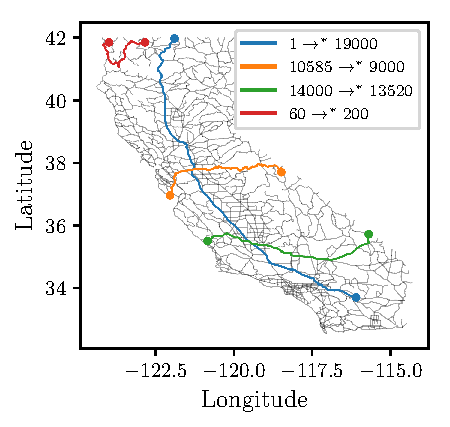
\includegraphics[scale=1]{figs/cal-node-paths.pdf}
    \caption{Four example shortest-paths in the Californian road network
        ($|V|=21048$, $|E|=21693$). These paths consist of
        575, 328, 272, and 207 nodes, respectively.
        % TODO next: Git commits, explain that make diagram, add all diagrams
        %    to GitHub as backup.
    }%
    \label{fig:cal-node-paths}%
    \vspace{-10pt}
\end{wrapfigure}

As an example, I have ran the algorithm on the graph in some above figure, and got
TODO. I have also done it on the Californian road network for four pairs of nodes,
deliberately picked to be either far apart or have a complicated shortest route
between them. Using the additional real-world data about all the nodes' longitude
and latitude, I have plotted the output of the \ac{MatSquare} algorithm in
\autoref{fig:cal-node-paths}.

\begin{figure}
    \centering
    \subfigure[Figure A]{%
        \label{fig:main-plot-fig-a}%
        % TODO: fix which plots are there
        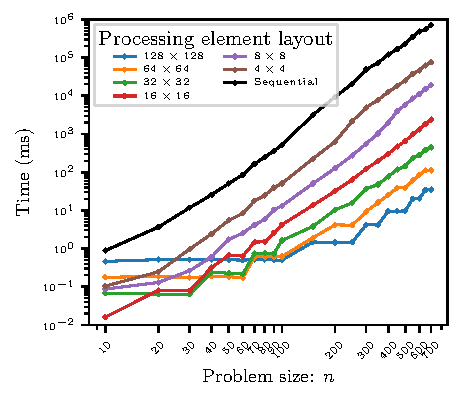
\includegraphics{figs/plots/total-time-scaling-sandy-full-width-no-errorbars.pdf}%
        \hfill%
        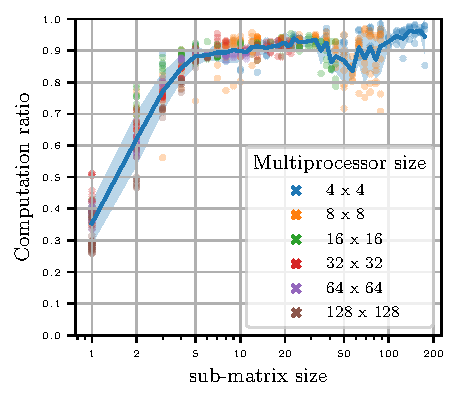
\includegraphics{figs/plots/ratio-bucket-sandy-half-scale.pdf}
    }%
    \vskip\baselineskip\vspace{-25pt}%
    \subfigure[Figure B]{%
        \label{fig:main-plot-fig-b}%
        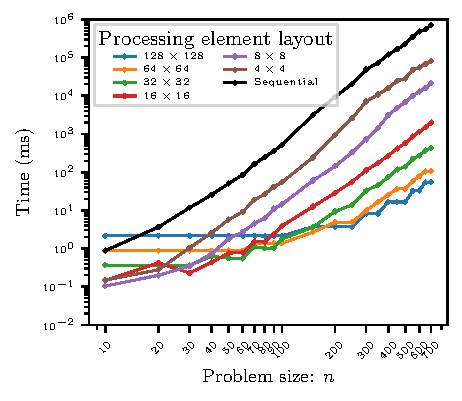
\includegraphics{figs/plots/total-time-scaling-taihu-full-width-no-errorbars.pdf}%
        \hfill%
        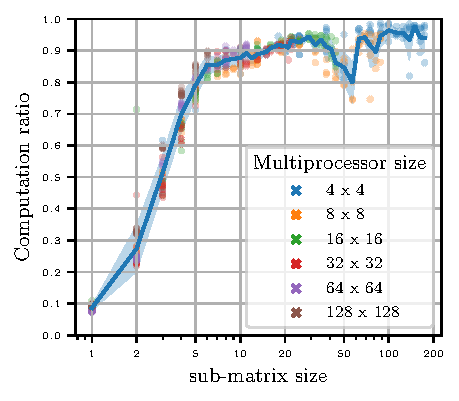
\includegraphics{figs/plots/ratio-bucket-taihu-half-scale.pdf}
    }%
    \vskip\baselineskip\vspace{-25pt}%
    \subfigure[Figure C]{%
        \label{fig:main-plot-fig-c}%
        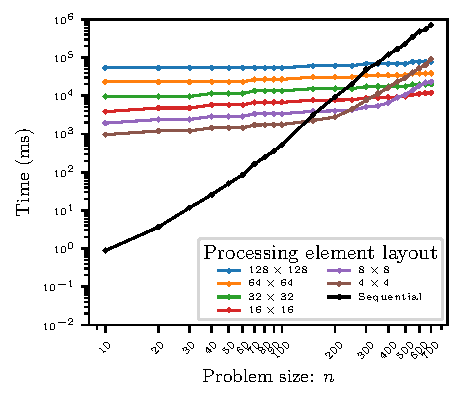
\includegraphics{figs/plots/total-time-scaling-internet-full-width-no-errorbars.pdf}%
        \hfill%
        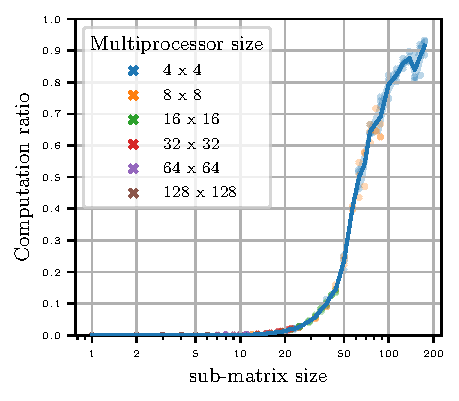
\includegraphics{figs/plots/ratio-bucket-internet-half-scale.pdf}
    }%
\caption{Global caption that might be a bit long as it goes over two lines, right
about now... It might even go over three lines since we are daring today. Just
this extra sentence should do it.}
\label{fig:main-eval-plot}
\end{figure}

\section{Evaluation metrics}

Nothing in this section

\section{Parallel matrix-multiplication}

\newpage
See \autoref{fig:example1} for some example plots. There is also
\autoref{fig:example3} which shows some stuff.


% Example figure
\begin{figure}
    \begin{center}
        % \includegraphics[scale=1]{figs/plots/example1.pdf}
        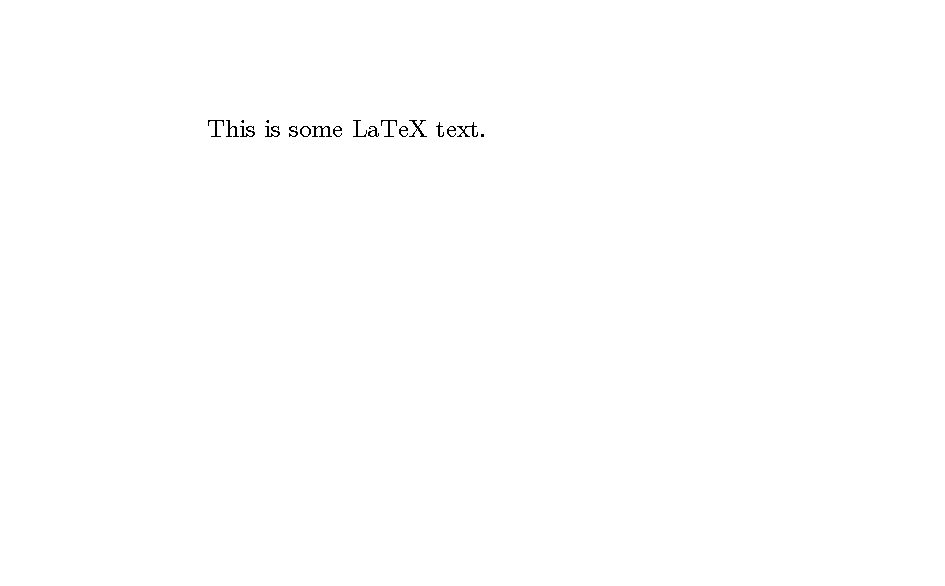
\includegraphics{inkscape-diagrams/template-diagram2.pdf}
    \end{center}
    \caption{Example diagram produced with inkscape}
    \label{fig:example1}
\end{figure}

% Comparison of computation ratio
\begin{figure}%
    \hfill
    \subfigure[Sandy bridge]{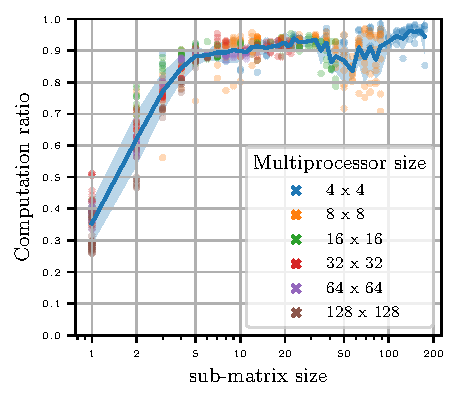
\includegraphics[scale=0.95]{figs/plots/ratio-bucket-sandy-half-scale.pdf}}
    \hfill
    \subfigure[Taihu light]{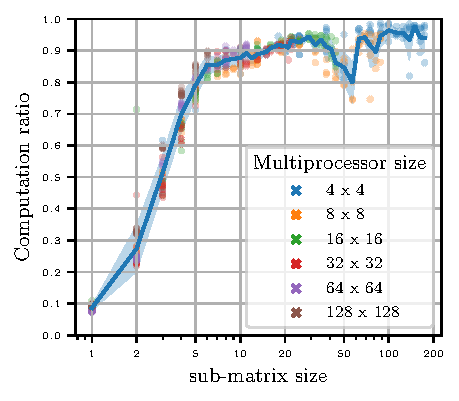
\includegraphics[scale=0.95]{figs/plots/ratio-bucket-taihu-half-scale.pdf}}
    \hfill
    \caption{Title for both, and explain some more...}
    \label{fig:example2}
\end{figure}

% Third example figure
\begin{figure}
    \begin{center}
        % \includegraphics[scale=1]{figs/plots/example3.pdf}
        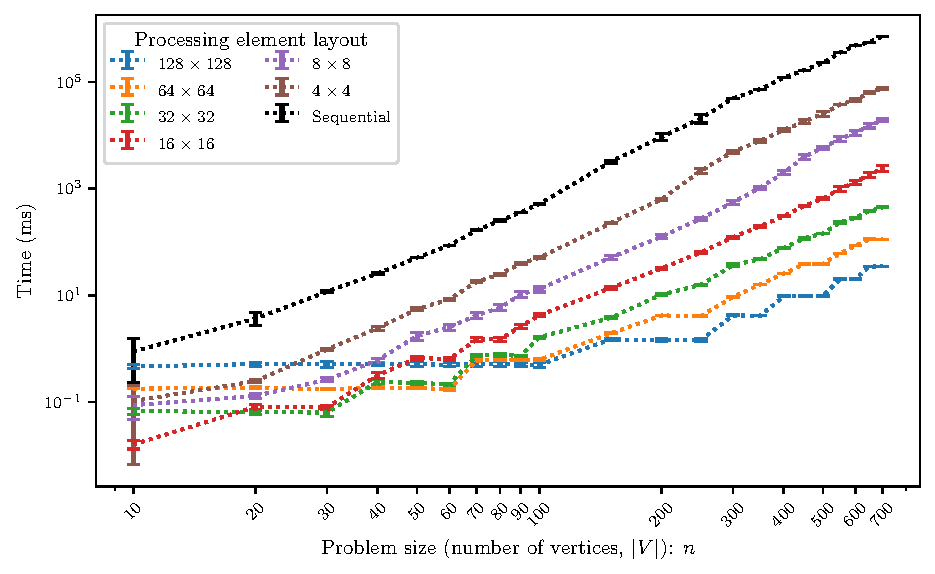
\includegraphics{figs/plots/total-time-scaling-sandy-full-width.pdf}
    \end{center}
    \caption{Sandy bridge total time scaling}
    \label{fig:example3}
\end{figure}

% Fourth example figure
\begin{figure}
    \begin{center}
        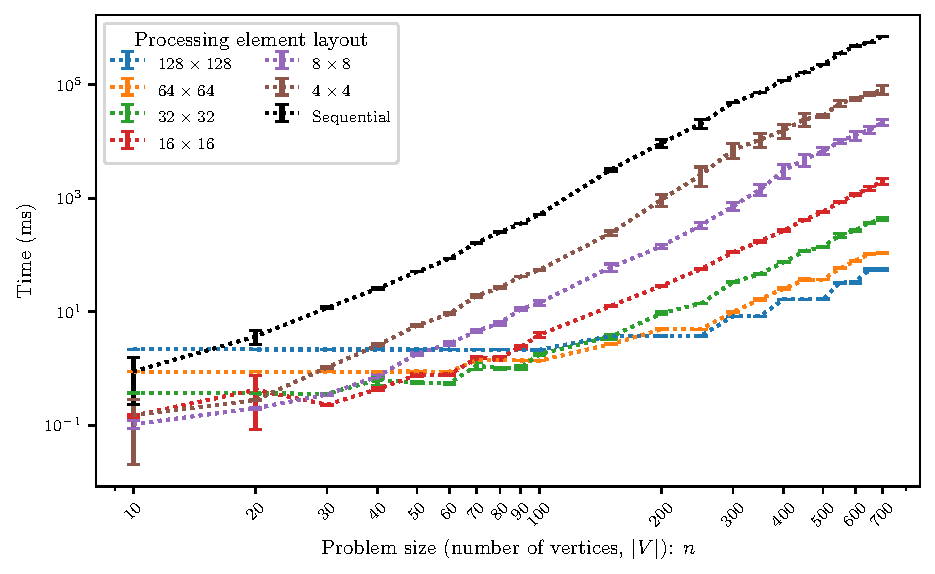
\includegraphics[scale=1]{figs/plots/total-time-scaling-taihu-full-width.pdf}
    \end{center}
    \caption{Taihu light total time scaling}
    \label{fig:example4}
\end{figure}


% Explanation of where constants from:
Bandwidth internet values based on report from \url{https://www.cable.co.uk/broadband/speed/worldwide-speed-league/}. Latency values for Europe based on statistics from
Verizon here \url{https://www.verizon.com/business/terms/latency/}. Chose round-trip
time because TCP transfer, and ACKs etc.
